\section{Использование коллекций}

\subsection{Условие задания}

Разработать приложение в соответствии со своим вариантом. Номер варианта выдает преподаватель. 

Приложение должно содержать следующие пункты:

\begin{enumerate}
    \item Заголовок формы должен отражать суть задания.
    \item Все элементы формы должны быть внятно подписаны (кнопки подписаны, у тестового поля должно быть написано, для чего оно нужно и т. д.)
    \item В коде должны быть комментарии и отступы (код должен быть легко читаем).
    \item В коде программы все элементы формы должны быть переименованы (btnName -  для кнопок, lblName - для ссылок, txtName - для текстового поля и т. д.) Наименования должны быть понятными.
    \item Должна быть возможность для ввода и вывода первоначальных данных.
    \item Должна быть возможность для вставки и удаления одного элемента.
    \item Должны использоваться коллекции.
    \item Ответы на задания должны быть в разных полях.
    \item Если нет данных для выполнения задания, выводить соответствующие данные.
    \item Для графов использовать список смежности.
\end{enumerate}

\textbf{Вариант 7.} Создать стек, состоящий из целых чисел. Предусмотреть возможность создания стека из набора чисел, добавления одного элемента (функция push), удаления одного элемента (функция pop), вывода результата на экран, удаления всех элементов с помощью кнопок. Найти максимальный нечетный элемент. Получить новый стек, удалив все нечетные элементы.


\subsection{Вид формы в конструкторе}



Для реализации стека создано окно приложения, содержащее пять элементов TextBox, три элемента Label, пять элементов Button и один элемент ErrorProvider для обработки ошибок. Вид окна представлен на рисунке \ref{task7_form} \cite{chang2021analysis}.
\begin{figure}[H]
    \centering
    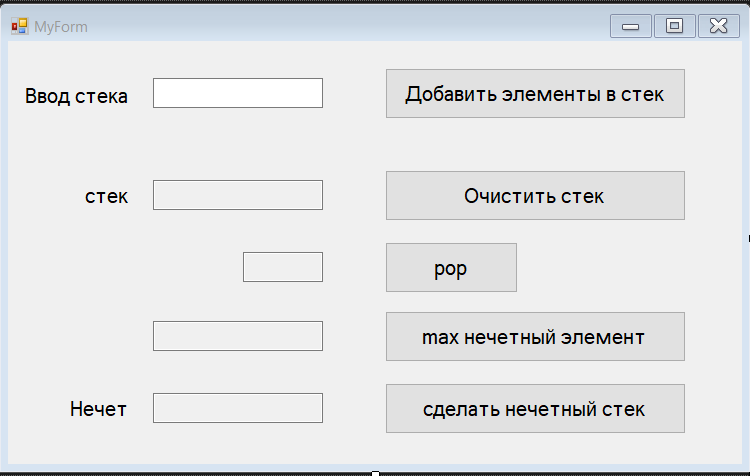
\includegraphics[width=1\linewidth]{lections/img/task7_form.png}
    \caption{Окно приложения «Матричный калькулятор» открытое в конструкторе}
    \label{task7_form}
\end{figure}



\subsection{Таблица с описанием переименованных элементов формы}
Все измененные элементы формы указаны в таблице \ref{task7_attributes}.


\begin{longtable}{|l|l|l|}
\caption{Значения атрибутов элементов в приложении <<Работа с коллекциями>>}\label{task7_attributes}\\
\hline
\textbf{\begin{tabular}[c]{@{}l@{}}Описание элементов\\ формы\end{tabular}}                                & \textbf{\begin{tabular}[c]{@{}l@{}}Список измененных\\ атрибутов\end{tabular}} & \textbf{\begin{tabular}[c]{@{}l@{}}Новое значение\\ атрибута\end{tabular}} \\ \hline
\endfirsthead
%
\endhead
%
Форма MyForm                                                                                               & Text                                                                           & Работа с коллекциями                                                       \\ \hline
TextBox ввода стека                                                                                        & Name                                                                           & input\_stack                                                               \\ \hline
\multirow{2}{*}{TextBox вывода стека}                                                                      & Name                                                                           & output                                                                     \\ \cline{2-3} 
                                                                                                           & ReadOnly                                                                       & True                                                                       \\ \hline
\multirow{2}{*}{\begin{tabular}[c]{@{}l@{}}TextBox вывода pop\\ элемента\end{tabular}}                     & Name                                                                           & pop\_out                                                                   \\ \cline{2-3} 
                                                                                                           & ReadOnly                                                                       & True                                                                       \\ \hline
\multirow{2}{*}{\begin{tabular}[c]{@{}l@{}}TextBox вывода максимального\\ нечетного элемента\end{tabular}} & Name                                                                           & max\_nech                                                                  \\ \cline{2-3} 
                                                                                                           & ReadOnly                                                                       & True                                                                       \\ \hline
\multirow{2}{*}{\begin{tabular}[c]{@{}l@{}}TextBox вывода стека из\\ нечетных элементов\end{tabular}}      & Name                                                                           & nech\_stack                                                                \\ \cline{2-3} 
                                                                                                           & ReadOnly                                                                       & True                                                                       \\ \hline
\multirow{2}{*}{\begin{tabular}[c]{@{}l@{}}Кнопка "Добавить элементы\\ в стек"\end{tabular}}               & Name                                                                           & create\_stack                                                              \\ \cline{2-3} 
                                                                                                           & Text                                                                           & \begin{tabular}[c]{@{}l@{}}Добавить элементы в\\ стек\end{tabular}         \\ \hline
\multirow{2}{*}{Кнопка "Очистить стек"}                                                                    & Name                                                                           & clear\_stack                                                               \\ \cline{2-3} 
                                                                                                           & Text                                                                           & Очистить стек                                                              \\ \hline
\multirow{2}{*}{Кнопка "pop"}                                                                              & Name                                                                           & pop\_stack                                                                 \\ \cline{2-3} 
                                                                                                           & Text                                                                           & pop                                                                        \\ \hline
\multirow{2}{*}{\begin{tabular}[c]{@{}l@{}}Кнопка "max нечетный \\ элемент"\end{tabular}}                  & Name                                                                           & max\_nech\_btn                                                             \\ \cline{2-3} 
                                                                                                           & Text                                                                           & max нечетный элемент                                                       \\ \hline
\multirow{2}{*}{\begin{tabular}[c]{@{}l@{}}Кнопка "Сделать нечетный\\ стек"\end{tabular}}                  & Name                                                                           & nech\_stack\_btn                                                           \\ \cline{2-3} 
                                                                                                           & Text                                                                           & сделать нечетный стек                                                      \\ \hline
\end{longtable}


\subsection{Примеры правильной и неправильной работы}
После запуска программы на экране появляется окно на рисунке \ref{task7_launch1}.
\begin{figure}[H]
    \centering
    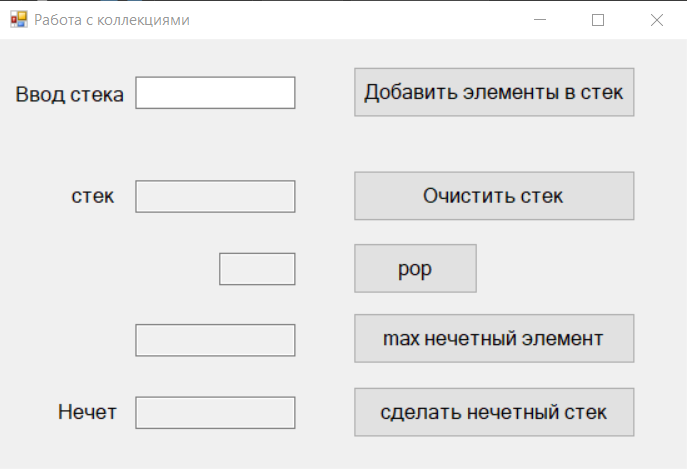
\includegraphics[width=0.8\linewidth]{lections/img/task7_launch1.png}
    \caption{Запуск программы}
    \label{task7_launch1}
\end{figure}

После ввода поле целых чисел через пробел и нажатии на кнопку "Добавить элементы в стек" (на рисунке \ref{task7_launch2}).

\begin{figure}[H]
    \centering
    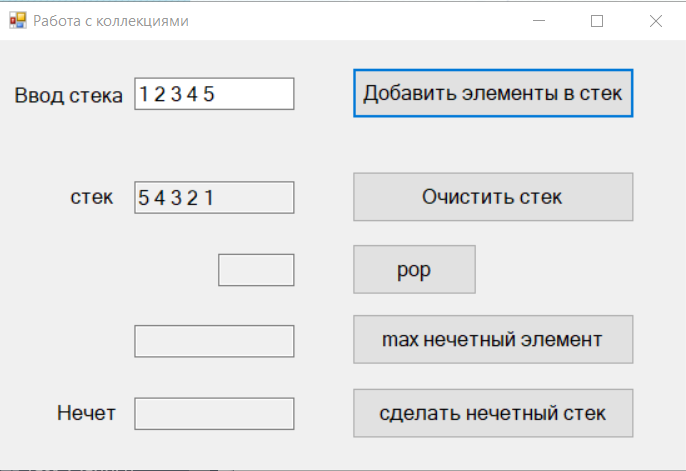
\includegraphics[width=0.8\linewidth]{lections/img/task7_launch2.png}
    \caption{Ввод стека}
    \label{task7_launch2}
\end{figure}

При попытке ввода не числа в поле, программа выведет ошибку (на рисунке \ref{task7_launch3})
\begin{figure}[H]
    \centering
    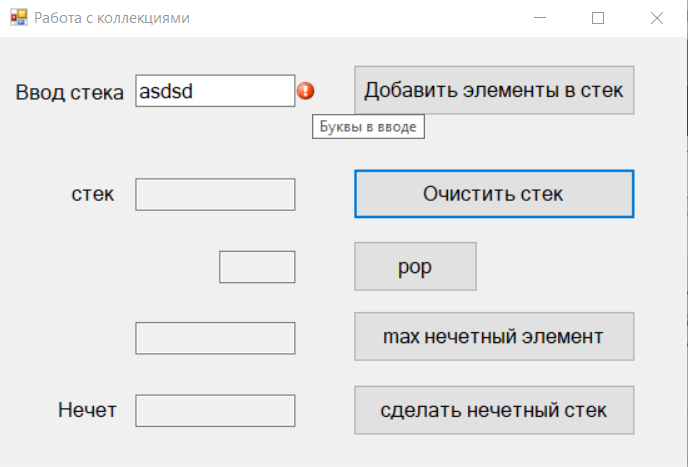
\includegraphics[width=0.8\linewidth]{lections/img/task7_launch3.png}
    \caption{Ошибка формата ввода}
    \label{task7_launch3}
\end{figure}



\subsection{Примеры исходного кода}


Функция очистки стека.
\begin{minted}[style=bw,
 linenos=true,
 breaklines=true,
 numbersep=5pt,
 tabsize=2,
 fontsize=\small,
 bgcolor=white]{cpp}
private: System::Void stack_out() {
	System::Collections::Generic::Stack<int> buf; //вспомогательный стек
	System::String^ str2 = "";
	while (s.Count) {//пока стек не пуст
		buf.Push(s.Peek()); //записываем во вспомогательный стек первый элемент
		str2 += System::Convert::ToString(s.Peek()) + " "; //записываем первый элемент в строку
		s.Pop(); //удаляем первый элемент из стека


	}
	while (buf.Count) { //пока вспомогательный стек не пуст
		s.Push(buf.Peek()); //записываем в основной стек первый элемент вспомогательного
		buf.Pop(); //удаляем из стека первый элемент

	}

	this->output->Text = str2; //записываем результат в строку
}
\end{minted}
Другие фрагменты кода расположены в приложении \ref{app:collections}.
\sectionbreak